\documentclass[12pt]{article}
\usepackage{amsmath,amssymb} % 数学环境
\usepackage{enumitem}      % 列表自定义
\usepackage{xcolor}        % 颜色
\usepackage[most]{tcolorbox}     % 答案块
\usepackage{geometry}      % 页边距
\geometry{a4paper, left=2.5cm, right=2.5cm, top=2.5cm, bottom=2.5cm}
\usepackage{fontspec}      % 使用系统字体
\usepackage{siunitx}
\usepackage{tabularray}
\usepackage{float}
\usepackage{siunitx}
\usepackage{fancyhdr}
\usepackage[hidelinks]{hyperref}
\usepackage{xurl}
\usepackage[normalem]{ulem}
\usepackage{graphics}
\usepackage{caption}
\usepackage{tabularx}
\usepackage{pdfpages}



\pagestyle{fancy}
\fancyhf{}
\fancyhead[L]{\textit{Solutions to End-of-Chapter Problems}}
\fancyfoot[C]{\thepage}          % 页脚居中页码


\setmainfont[
  Path = Font/,          % 字体路径
  UprightFont = *-Regular.ttf,       % 正文字体
  ItalicFont = *-Italic.ttf,         % 斜体
  BoldFont = *-Bold.ttf,             % 粗体
  BoldItalicFont = *-BoldItalic.ttf,  % 粗斜体
  Ligatures=TeX
]{EBGaramond}

\newfontfamily\titlefont[
  Path = Font/,
  UprightFont = *-Regular.ttf,
  ItalicFont = *-Italic.ttf,         % 斜体
  BoldFont = *-Bold.ttf,             % 粗体
  BoldItalicFont = *-BoldItalic.ttf,  % 粗斜体
  Numbers = OldStyle,
  Ligatures = {Historic,Rare,Common,Contextual},
]{EBGaramond}


\usepackage{unicode-math}
\setmathfont[Path = Font/, ]{Garamond-Math.otf}
% 定义题号宽度变量,保证不同长度题号正文对齐
\newlength{\questionlabelwidth}
\setlength{\questionlabelwidth}{2.5em} % 根据最大题号长度调整

\newcommand{\question}[2]{%
  \par\noindent
  {\hangindent=2.5em % 悬挂缩进
   \hangafter=1 % 从第一行起生效
   \makebox[\questionlabelwidth][l]{\textbf{#1}}#2\par}%
}

\definecolor{BPink}{RGB}{242, 62, 112}

% 答案块:莫兰迪蓝风格
\definecolor{morandiBlue}{RGB}{160,175,190} % 柔和蓝灰
\definecolor{morandiBorder}{RGB}{120,140,160} 
\definecolor{moranblue}{RGB}{58, 80, 107}
\definecolor{outerGray}{RGB}{180,180,180}

\newtcolorbox{answerbox}{
  enhanced,        % 启用高级功能
  breakable,       % 可跨页    
  colback=morandiBlue!20,          
  colframe=outerGray,          % 边框色
  colbacktitle=morandiBorder,      % 标题背景:米白
  fonttitle=\bfseries,
  title=ANSWER,
  boxrule=1pt,
  arc=0pt,
  left=4mm,
  right=4mm,
  top=2mm,
  bottom=2mm,
  title after break={ANSWER},
  overlay={                     % 外层灰色边框
    \draw[outerGray,line width=1.2pt]
      (frame.south west) rectangle (frame.north east);
  },
}

% Morandi灰绿系配色
\definecolor{morandiGreen}{RGB}{120, 135, 120}   % 深灰绿(边框)
\definecolor{morandiLightGreen}{RGB}{220, 228, 220} % 淡灰绿(背景)
\definecolor{morandiOlive}{RGB}{150, 140, 120}   % 柔和橄榄灰(标题文字)
\definecolor{morandiIvory}{RGB}{245, 242, 236}   % 米白(标题背景)

% Morandi灰绿系 answerboxq
\newtcolorbox{answerboxq}{
    enhanced,
    breakable,
    colback=morandiLightGreen,      % 背景:浅灰绿
    colframe=morandiGreen,          % 边框:深灰绿
    colbacktitle=morandiIvory,      % 标题背景:米白
    coltitle=morandiOlive,          % 标题文字:橄榄灰
    fonttitle=\bfseries,      % 标题加粗
    title=ANSWER,
    title after break={ANSWER},       % 跨页标题重复
    arc=0pt,                        % 圆角
    boxrule=1pt,
    left=4mm, right=4mm, top=2mm, bottom=2mm,
    overlay={                     % 外层灰色边框
    \draw[morandiGreen,line width=1.2pt]
      (frame.south west) rectangle (frame.north east);
    }

}

\newcommand{\vect}[1]{\boldsymbol{\mathbf{#1}}}
\newcommand{\pp}[1]{#1^{\prime}}
\newcommand{\ReN}{\mathrm{Re}}


\captionsetup{
    labelformat=empty,       % 去掉编号
    font=bf,
    justification=centering
}

\DeclareSIUnit{\Fahrenheit}{\text{\textdegree F}}
\DeclareSIUnit{\Rankine}{\text{\textdegree R}}

% 自定义链接命令(长链接可自动换行,保留蓝色)
\newcommand{\mylink}[2]{%
  \href{#1}{\textcolor{moranblue}{\textit{#2}}}%
}

\begin{document}

\thispagestyle{empty}

\includepdf[pages=1]{cover.pdf}

\newpage

\thispagestyle{empty}

\tableofcontents

\newpage

\setcounter{page}{1}

\section*{Document Introduction}
\addcontentsline{toc}{section}{0 \hspace{0.5em} Document Introduction} % 手动加入目录

This document is typeset using \LaTeX. I only handled the typesetting and partial proofreading, \textcolor{red}{so some answers may contain errors}. Please verify them yourself.  

If you need the \LaTeX\ source code, please visit this Github repository: \mylink{https://github.com/RLee0310/Answer-for-XMU-Fundamentals-of-Gas-Dynamics/tree/main}{Answer} to gain the source code.  

I would like someone to continue updating this document. If anyone has ideas in this area, you can contact me via email to become a contributor to this repository.

\textbf{My email address:} 

GMail: \quad \mylink{mailto: amourse81@gmail.com}{amourse81@gmail.com}.

Outlook: \mylink{mailto: RebeccaLee0310@outlook.com}{RebeccaLee0310@outlook.com}

It should be noted that students in China cannot directly access GitHub, so you may need to use circumvention tools (like a VPN or proxy) to access it.

Here I would like to recommend \mylink{https://www.keepresearch.com}{Keepresearch}, which is a free online \LaTeX\ editor. Compared with Overleaf, it is more suitable for Chinese students.
This project, including the source code, is also available on \textit{Keepresearch}. If you wish to use \textit{Keepresearch} to edit the document, you can also contact me via email.

The document uses \textbf{EB Garamond} as the main font. EB Garamond is an elegant classical serif font, but for Chinese students, reading it may be somewhat challenging.  
Here we list all the English upright letters, italic letters and Greek letters in EB Garamond for easier reference.

\begin{center}
\Large \textcolor{BPink}{\textbf{Hope you all achieve good grades in this course.}}
\end{center}

\subsection*{English Letters}

\noindent\textbf{Upright:}

ABCDEFGHIJKLMNOPQRSTUVWXYZ\\
\indent abcdefghijklmnopqrstuvwxyz\\[0.5em]

\noindent\textbf{Italic:}

\textit{ABCDEFGHIJKLMNOPQRSTUVWXYZ}\\
\indent\textit{abcdefghijklmnopqrstuvwxyz}

%---------------------------------
% 2. Greek Letters (Math Mode)
%---------------------------------
\subsection*{Greek Letters}

% \usepackage{tabularray}
% \usepackage{tabularray}
\begin{longtblr}[
  label = none,
  entry = none,
]{
  width = \linewidth,
  colspec = {Q[183]Q[290]Q[267]Q[194]},
  cells = {c},
  vlines,
  hline{1-2,26} = {-}{},
   rowhead = 1,             % 重复表头
}
\textbf{Letter Name} & \textbf{Lowercase (upright)} & \textbf{Lowercase Variant} & \textbf{Uppercase} \\
Alpha                & $\alpha$                     & -                          & $\Alpha$           \\
Beta                 & $\beta$                      & -                          & $\Beta$            \\
Gamma                & $\gamma$                     & -                          & $\Gamma$           \\
Delta                & $\delta$                     & -                          & $\Delta$           \\
Epsilon              & $\epsilon$                   & $\varepsilon$              & $\Epsilon$         \\
Zeta                 & $\zeta$                      & -                          & $\Zeta$            \\
Eta                  & $\eta$                       & -                          & $\Eta$             \\
Theta                & $\theta$                     & $\vartheta$                & $\Theta$           \\
Iota                 & $\iota$                      & -                          & $\Iota$            \\
Kappa                & $\kappa$                     & -                          & $\Kappa$           \\
Lambda               & $\lambda$                    & -                          & $\Lambda$          \\
Mu                   & $\mu$                        & -                          & $\Mu$              \\
Nu                   & $\nu$                        & -                          & $\Nu$              \\
Xi                   & $\xi$                        & -                          & $\Xi$              \\
Omicron              & $\omicron$                   & -                          & $\Omicron$         \\
Pi                   & $\pi$                        & $\varpi$                   & $\Pi$              \\
Rho                  & $\rho$                       & $\varrho$                  & $\Rho$             \\
Sigma                & $\sigma$                     & $\varsigma$                & $\Sigma$           \\
Tau                  & $\tau$                       & -                          & $\Tau$             \\
Upsilon              & $\upsilon$                   & -                          & $\Upsilon$         \\
Phi                  & $\phi$                       & $\varphi$                  & $\Phi$             \\
Chi                  & $\chi$                       & -                          & $\Chi$             \\
Psi                  & $\psi$                       & -                          & $\Psi$             \\
Omega                & $\omega$                     & -                          & $\Omega$           
\end{longtblr}



\newpage

\section{Chapter 1}

\question{1.1}{Given that standrad atmosphere conditions for air at 15\,\si{\celsius} are a pressure of 1.013 \,\si{bar} and
a density of 1.225\,\si{kg}, calculate the gas constant for air.}

\begin{answerbox}
It follows from $P=\rho RT$ that $R=\dfrac{\rho T}{P}=\dfrac{1.013\times 10^5}{(15+273)\times 1.225}=287.13$\,\si{\joule/(\kilogram\cdot\kelvin)}.
\end{answerbox}

\question{1.2}{The value of $C_v$ for air is 717\,\si{J/(kg\cdot K)}. The value of $R=287$\,\si{J/(kg\cdot K)}. Calculate the specific enthalpy of air
at 20\,\si{\celsius}. Derive a relation connecting $C_p$, $C_v$, $R$. Use this relation to calculate Cp for air using the information above.}

\begin{answerbox}
Consider a gas of unit mass as an example.

$h=u+pv=u+\rho RTv=u+RT$.

and $C_p$ define as $C_p=\dfrac{\partial h}{\partial T}$ and $C_v=\dfrac{\partial u}{\partial T}$, so we obtain:

$C_p=\dfrac{\partial h}{\partial T}=\dfrac{\partial u}{\partial T}+mR=C_v+mR=C_v+R$.

Thus, $C_p=717+287=1.004$\,\si{kJ/(kg\cdot K)}.

so $h=C_pT=1.004\times (20+273)=294.3$\,\si{kJ/kg}.
\end{answerbox}

\question{1.3}{Air is stored in a cylinder at a pressure of 10 \,\si{bar}, and at a room temperature of 25\,\si{\celsius}. How much
volume will 1\,\si{kg} of air occupy inside the cylinder? The cylinder is rated for a maximum pressure of 15 \,\si{bar}. At what temperature would this pressure be reached?}

\begin{answerbox}
It follows from $P=\rho RT=\dfrac{m}{V}RT$ that:

$V=\dfrac{mRT}{P}=\dfrac{1\times 287\times (25+273)}{10\times 10^5}=0.086$\,\si{m^3}.

From $\dfrac{P_1}{P_2}=\dfrac{T_1}{T_2}$,we obtain:

$T_2=T_1\dfrac{P_2}{P_1}=298\times \dfrac{15}{10}=447$\,\si{K}.
\end{answerbox}

\question{1.4}{Derive the follow formulations from basic thermodynamics equations learned in this lecture,
\begin{align*}
  &s_2-s_1=c_v\ln\left[\dfrac{T_2}{T_1}\right]+R\ln\left[\dfrac{\rho_1}{\rho_2}\right] &\dfrac{T_2}{T_1}=\left[\exp\dfrac{s_2-s_1}{c_v}\right]\left(\dfrac{\rho_2}{\rho_1}\right)^{R/c_v} \\
  &s_2-s_1=c_p\ln\left[\dfrac{T_2}{T_1}\right]-R\ln\left[\dfrac{P_2}{P_1}\right] &\dfrac{T_2}{T_1}=\left[\exp\dfrac{s_2-s_1}{c_p}\right]\left(\dfrac{P_2}{P_1}\right)^{R/c_p}
\end{align*}
}
\begin{answerbox}
From the definition of entropy, we have: $ds=\dfrac{\delta q}{T}=\dfrac{dh-vdp}{T}$,

so that: $Tds=dh-vdp$.

Since $du=c_vdT$, $dh=c_pdt$, we obtain: $Tds=c_vdT+pdv=c_pdT-vdp$.

Integrating the above equation yields the expression on the left, which can also be transformed into the expression on the right.
\end{answerbox}

\newpage

\section{Chapter 2}
\question{2.4}{Evaluate the integal $\int\rho e\left(\vect{V}\cdot \hat{n}\right)dA$ over the surface shown in Figure P2.4 for the velocity and energy distributions indicated. Assume that the density is constant.

\begin{figure}[H]
  \centering
  \includegraphics[width=0.5\textwidth]{pic/P2.4.png}
  \caption{Figure P2.4}
\end{figure}
}

\begin{answerbox}
\begin{align*}
  \int\rho e(\vect{V}\cdot \hat{n})dA &=\int\rho E_{max}\left(1-\dfrac{A}{A_0}\right)V_{\max}\left(1-\dfrac{A}{A_0}\right)dA \\
  &=\rho E_{max}V_{max}\int_0^{A_0}\left(1-\dfrac{A}{A_0}\right)^2dA \\
  &=\dfrac{1}{3}\rho E_{mac}V_{max}A_0
\end{align*}
\end{answerbox}

\question{2.6}{Nitrogen flows in a constant-area duct. Conditions at section 1 are as follows: $p_1=200$\,\si{psia}, $T_1=90$\,\si{\Fahrenheit}, and $V_1=10$\,\si{ft/sec}. At section 2, we find that $p_2=45$\,\si{psia} and $T_2=90$\,\si{\Fahrenheit}. Determine the velocity at section 2.}

\begin{answerbox}
From the continuity equation, we have $\rho_1V_1A_1=\rho_2V_2A_2$.

And $P=\rho RT$, so that $\rho=\dfrac{P}{RT}$.

Thus, we obtain $V_2=V_1\dfrac{P_1T_2}{P_2T_1}=10\times \dfrac{200\times (90+460)}{45\times (90+460)}=44.44$\,\si{ft/sec}.
\end{answerbox}

\question{2.9}{Hydrogen expands isentropically from $15$\,\si{bar} absolute and $340$\,\si{K} to $3$\,\si{bar} absolute in a steady flow process without heat transfer.\\
(a)	Compute the final velocity if the initial velocity is negligible.\\
(b)	Compute the flow rate if the final duct size is $10$\,\si{cm} in diameter.
}

\begin{answerbox}
(a) Since $V_1=0$, $w_s=0$, $z_1=z_2$, from $h_1+\dfrac{V_1^2}{2}+gz_1=h_2+\dfrac{V_2^2}{2}+gz_2+w_s$, we obtain:

$V_2=\sqrt{2(h_1-h_2)}=\sqrt{2c_p(T_1-T_2)}$.

And as the gas is Hydrogen, so that $R=4147$\,\si{J/(kg\cdot K)}, $c_p=14.05$\,\si{J/(kg\cdot K)}.

From the isentropic relation, we have: $\Delta s_{1-2}=c_p\ln\dfrac{T_2}{T_1}-R\ln\dfrac{P_2}{P_1}=0$, thus $T_1=211.2$\,\si{K}.

Thus $V_2=1902$\,\si{m/s}.

(b) $Q=\rho V_2A=\dfrac{P_2}{RT_2}V_2A=5.1$\,\si{kg/s}.
\end{answerbox}

\question{2.14}{Cold water with an enthalpy of $8$\,\si{Btu/lbm} enters a heater at the rate of $5$\,\si{lbm/sec} with a velocity of $10$\,\si{ft/sec} and at a potential of $10$\,\si{ft} with respect to the other connections shown in Figure P2.14. Steam enters at the rate of $1$\,\si{lbm/sec} with a velocity of $50$ \,\si{ft/sec} and an enthalpy of $1350$\,\si{Btu/lbm}. These two streams mix in the heater, and hot water emerges with an enthalpy of $168$\,\si{Btu/lbm} and a velocity of $12$\,\si{ft/sec}.\\
(a)	Determine the heat lost from the apparatus.\\
(b)	What percentage error is involved if both kinetic and potential energy changes are neglected?
\begin{figure}[H]
  \centering
  \includegraphics[width=0.5\textwidth]{pic/P2.14.png}
  \caption{Figure P2.14}
\end{figure}
}

\begin{answerbox}
(a) From the steady flow energy equation, we have:
\[
\dot{m_1}\left(h_1+\dfrac{V_1^2}{2g_c}+\dfrac{g}{g_c}z_1\right)+\dot{m_2}\left(h_2+\dfrac{V_2^2}{2g_c}+\dfrac{g}{g_c}z_2\right)+\dot{Q}=\left(\dot{m_1}+\dot{m_2}\right)\left(h_3+\dfrac{V_3^2}{2g_c}+\dfrac{g}{g_c}z_3\right)+w_s
\]
And $z_1=10$\,\si{ft}, $z_2=0$\,\si{ft}, $z_3=0$\,\si{ft}, $V_1=10$\,\si{ft/sec}, $V_2=50$\,\si{ft/sec}, $V_3=12$\,\si{ft/sec}, $h_1=8$\,\si{Btu/lbm}, $h_2=1350$\,\si{Btu/lbm}, $h_3=168$\,\si{Btu/lbm}, $\dot{m_1}=5$\,\si{lbm/sec}, $\dot{m_2}=1$\,\si{lbm/sec}.

Thus, we obtain $\dot{Q}=382.1$\,\si{Btu/sec}.

(b) Neglecting the kinetic and potential energy changes, we have:
\[
\dot{m_1}h_1+\dot{m_2}h_2+\dot{Q^\prime}=\left(\dot{m_1}+\dot{m_2}\right)h_3+w_s
\]
Thus, we obtain $\dot{Q^\prime}=382$\,\si{Btu/sec}.

So the percentage error is $\dfrac{|\dot{Q}-\dot{Q^\prime}|}{\dot{Q}}\times 100\%=0.03\%$.

\end{answerbox}

\question{2.15}{The control volume shown in Figure P2.15 has steady, incompressible flow and all properties are uniform at the inlet and outlet. For $u_1 = 1.256$\,\si{MJ/kg} and $u2 = 1.340$\,\si{MJ/kg} and $\rho=10$\,\si{kg/m^3}, calculate the work if there is a heat output of $0.35$\,\si{MJ/kg}.
\begin{figure}[H]
  \centering
  \includegraphics[width=0.5\textwidth]{pic/P2.15.png}
  \caption{Figure P2.15}
\end{figure}
}

\begin{answerbox}
Since $q=w_s+(e_2+p_2v_2)-(e_1+p_1v_1)$, and $e=u+\dfrac{V^2}{2}+gz$.

And $v_1=v_2=\dfrac{1}{\rho}=0.1$\,\si{m^3/kg}, $q=-0.35$\,\si{MJ/kg}.

So we have $w_s=-0.434$\,\si{MJ/kg}.
\end{answerbox}

\newpage

\section{Chapter 3}
\question{3.6}{The following information is known about the steady flow of methane through a hori- zontal insulated duct:\\
\begin{align*}
&\text{Entering stagnation enthalpy} &= &634\,\si{Btu/lbm}\\
&\text{Leaving static enthalpy} &= &532\,\si{Btu/lbm}\\
&\text{Leaving static temperature} &= &540\,\si{\Fahrenheit}\\
&\text{Leaving static pressure} &= &50\,\si{psia}
\end{align*}
(a)	Determine the outlet velocity.\\
(b)	What is the stagnation temperature at the outlet?\\
(c)	Determine the stagnation pressure at the outlet.
}

\begin{answerbox}
(a) Since $h_t=h+\dfrac{V^2}{2g_c}+\dfrac{g}{g_c}z$, that $V_t=2260$\,\si{ft/sec}.

(b) As $h=c_p T$, $h_t=c_p T_t$, we obtain: $T_t=\dfrac{h_t}{c_p}=\dfrac{h_t T}{h}$.

And $T=540\,\si{\Fahrenheit}=1000\,\si{\Rankine}$, so $T_t=1191.73\,\si{\Rankine}=731.73\,\si{\Fahrenheit}$.

(c) From $\dfrac{p_t}{p}=\left(\dfrac{T_t}{T}\right)^{\frac{\gamma}{\gamma -1}}$, $\gamma = 1.32$, we obtain $p_t=103.18$\,\si{psia}.
\end{answerbox}

\question{3.18}{3.18.	Seawater ($\rho = 64$\,\si{lbm/ft^3}) flows through the reducer shown in Figure P3.18 with $p_1 =50$\,\si{psig}. The flow losses between the two sections amount to $h_l = 5.0$\,\si{ft-1bf/lbm}.\\
(a) Find $V_2$ and $p_2$.\\
(b)	Determine the force exerted by the reducer on the seawater between sections 1 and 2.
\begin{figure}[H]
  \centering
  \includegraphics[width=0.5\textwidth]{pic/P3.18.png}
  \caption{Figure P3.18}
\end{figure}
}

\begin{answerbox}
(a) Since $\dfrac{p_1}{\rho}+\dfrac{V_1^2}{2g_c}+\dfrac{g}{g_c}z_1=\dfrac{p_2}{\rho}+\dfrac{V_2^2}{2g_c}+\dfrac{g}{g_c}z_2+h_l$, $\rho A_1V_1=\rho A_2V_2$,

$V_2=80$\,\si{ft/sec}, $p_2=6.37$\,\si{psig}.

(b) From $F_x=\dfrac{\dot{m}}{g_c}(V_2-V_1)$, we obtain: $p_1A_1-p_2A_2-F_f=\dfrac{\rho A_1V_1}{g_c}(V_2-V_1)$.

Thus $F_f=3600$\,\si{lbf}.
\end{answerbox}

\question{3.19}{(a) Neglect all losses and compute the exit velocity from the tank shown in Figure P3.19.\\
(b)	If the opening is $4$\,\si{in.} in diameter, determine the mass flow rate.\\
(c)	Compute the force tending to push the tank along the floor.
\begin{figure}[H]
  \centering
  \includegraphics[width=0.5\textwidth]{pic/P3.19.png}
  \caption{Figure P3.19}
\end{figure}
}

\begin{answerbox}
(a) Since $\dfrac{p_1}{\rho}+\dfrac{V_1^2}{2g_c}+\dfrac{g}{g_c}z_1=\dfrac{p_2}{\rho}+\dfrac{V_2^2}{2g_c}+\dfrac{g}{g_c}z_2$, that $V_2=32.1$\,\si{ft/sec}.

(b) $\dot{m}=\rho AV_2=174.9$\,\si{lbm/sec}.

(c) $F_x=\dfrac{\dot{m}}{g_c}(V_{2x}-V_{1x})=\dfrac{\dot{m}}{g_c}V_2\cos\ang{30}=151$\,\si{lbf}.
\end{answerbox}

\newpage

\section{Chapter 4}
\question{4.5}{If $\gamma=1.2$ and the fluid is a perfect gas, what Mach number will give a temperature ratio of $T /T_t = 0.909$? What will the ratio of $p/p_t$ be for this flow?}

\begin{answerbox}
Since $T_t=T\left(1+\dfrac{\gamma -1}{2}M^2\right)$, thus $M=1$.

And $p_t=p\left(1+\dfrac{\gamma -1}{2}M^2\right)^{\frac{\gamma}{\gamma -1}}$, so $\dfrac{p}{p_t}=0.564$.
\end{answerbox}

\question{4.6}{Carbon dioxide with a temperature of $335$\,\si{K} and a pressure of $1.4\times 10^5$\,\si{N/m^2} is flowing with a velocity of $200$\,\si{m/s}.\\
(a) Determine the sonic velocity and Mach number.\\
(b) Determine the stagnation density.
}

\begin{answerbox}
(a) For Carbon dioxide $\gamma = 1.29$, $R=189$\,\si{N\cdot m/(kg\cdot K)}, and $T=335$\,\si{K}.

So $a=\sqrt{\gamma RT}=286$\,\si{m/s}, $M=\dfrac{V}{a}=0.7$.

(b) $p_t=p\left(1+\dfrac{\gamma -1}{2}M^2\right)^{\frac{\gamma}{\gamma -1}}=185546$\,\si{Pa}.

$T_t=T\left(1+\dfrac{\gamma -1}{2}M^2\right)=359$\,\si{K}.

Since $P_t=\rho_t R T_t$, thus $\rho_t=\dfrac{P_t}{RT}=2.73$\,\si{kg/m^3}.

\end{answerbox}

\question{4.11}{A large chamber contains a perfect gas under conditions $p_1$, $T_1$, $h_1$, and so on. The gas is allowed to flow from the chamber (with $q = w_s = 0$). Show that the velocity cannot be greater than\\
\begin{align*}
V_{\max}=a_1\left(\dfrac{2}{\gamma -1}\right)^{1/2}
\end{align*}
If the velocity is the maximum, what is the Mach number?
}

\begin{answerbox}
From $h_{t1}+q=h_{t2}+w_s$, and $q=w_s=0$, thus $h_{t1}=h_{t2}$, so that $T_{t1}=T_{t2}$.

And we obtain $T_1\left(1+\dfrac{\gamma -1}{2}M_{a1}^2\right)=T_2\left(1+\dfrac{\gamma -1}{2}M_{a2}^2\right)$.

As $M_{a1}=\dfrac{V_1}{a_1}=\dfrac{V_1}{\sqrt{\gamma RT_1}}$, $M_{a2}=\dfrac{V_2}{a_2}=\dfrac{V_2}{\sqrt{\gamma RT_2}}$,

So that $V_2=\sqrt{\dfrac{2(T_1-T_2)g_c\gamma R}{\gamma -1}}\leqslant \sqrt{\dfrac{2T_1g_c\gamma R}{\gamma -1}}=a_1\sqrt{\dfrac{2}{\gamma -1}}$.

That is $V_{\max}=a_1\sqrt{\dfrac{2}{\gamma -1}}$.

At this time $T_2=0$, thus $M_{a2}\to \infty$.
\end{answerbox}

\question{4.13}{Methane gas flows in an adiabatic, no-work system with negligible change in potential. At one section $p_1 = 14$\,\si{bar} abs., $T_1 = 500$\,\si{K}, and $V_1 = 125$\,\si{m/s}. At a downstream section $M_2 = 0.8$.\\
(a) Determine $T_2$ and $V_2$.\\
(b) Find $p_2$ assuming that there are no friction losses.\\
(c) What is the area ratio $A_2/A_1$?
}

\begin{answerbox}
(a) From $h_{t1}+q=h_{t2}+w_s$, and $q=w_s=0$, thus $h_{t1}=h_{t2}$, so that $T_{t1}=T_{t2}$.

And we obtain $T_1\left(1+\dfrac{\gamma -1}{2}M_{a1}^2\right)=T_2\left(1+\dfrac{\gamma -1}{2}M_{a2}^2\right)$.

As $T_1=500$\,\si{K}, $M_{a1}=\dfrac{V_1}{a_1}=\dfrac{V_1}{\sqrt{\gamma RT_1}}=0.21$, $M_{a2}=\dfrac{V_2}{a_2}=\dfrac{V_2}{\sqrt{\gamma RT_2}}=0.8$.

So that $T_2=457$\,\si{K}, $a_2=559$\,\si{m/s}, $V_2=a_2M_{a2}=448$\,\si{m/s}.

(b) Because There are no friction losses,  $p_1\left(1+\dfrac{\gamma -1}{2}M_{a1}^2\right)^{\frac{\gamma}{\gamma -1}}=p_2\left(1+\dfrac{\gamma -1}{2}M_{a2}^2\right)^{\frac{\gamma}{\gamma -1}}$.

So $p_2=9.65$\,\si{bar}.

(c) From continuity equation $\rho A_1 V_1=\rho A_2 V_2$, $\dfrac{A_2}{A_1}=0.37$.
\end{answerbox}

\newpage

\section{Chapter 5}
\question{5.1}{5.1.	The following information is common to each of parts (a) and (b). Nitrogen flows through a diverging section with $A_1 = 1.5$\,\si{ft^2} and $A_2 = 4.5$\,\si{ft^2}. You may assume steady, one- dimensional flow, $Q=W_s=0$, negligible potential changes, and no losses.\\
(a)	If $M_1 = 0.7$ and $p_1 = 70$\,\si{psia}, find $M_2$ and $p_2$.\\
(b)	If $M_1 = 1.7$ and $T_1 = 95$\,\si{\Fahrenheit}, find $M_2$ and $T_2$.
}

\begin{answerbox}
For there are no losses, $A_1^{*}=A_2^{*}, P_{t1}=P_{t2}, T_{t1}=T_{t2}$.

(a) As $M_1=0.7$, check the table we gain $\dfrac{A_1}{A_1^{*}}=1.094$.

So $\dfrac{A_2}{A_2^{*}}=\dfrac{A_2}{A_1}\dfrac{A_1}{A_1^{*}}\dfrac{A_1^{*}}{A_2^{*}}=3.238$, so $M_2=0.18$.

Thus $p_2=\dfrac{p_2}{p_{t2}}\dfrac{p_{t2}}{p_{t1}}\dfrac{p_{t1}}{p_1}p_1=94.9$\,\si{psia}.

(b) As $M_1=1.7$, check the table we gain $\dfrac{A_1}{A_1^{*}}=1.337$.

So $\dfrac{A_2}{A_2^{*}}=\dfrac{A_2}{A_1}\dfrac{A_1}{A_1^{*}}\dfrac{A_1^{*}}{A_2^{*}}=4.011$, so $M_2=2.94$.

Thus $T_2=\dfrac{T_2}{T_{t2}}\dfrac{T_{t2}}{T_{t1}}\dfrac{T_{t1}}{T_1}T_1=94.9$\,\si{\Fahrenheit}.
\end{answerbox}

\question{5.2}{Air enters a converging section where $A1 = 0.50$\,\si{m^2}. At a downstream section $A2 = 0.25$\,\si{m^2}, $M_2=1.0$, and $\Delta s_{1-2}=0$. It is known that $p_2 < p_1$. Find the initial Mach number ($M_1$) and the temperature ratio ($T_2/T_1$).
}

\begin{answerbox}
For $\Delta s_{1-2}=0$, $A_1^{*}=A_2^{*}, T_{t1}=T_{t2}$.

As $M_2=1.0$, check the table we gain $\dfrac{A_2}{A_2^{*}}=1.000$.

So $\dfrac{A_1}{A_1^{*}}=\dfrac{A_1}{A_2}\dfrac{A_2}{A_2^{*}}\dfrac{A_2^{*}}{A_1^{*}}=2.000$, so $M_1=2.2$.

Thus $\dfrac{T_2}{T_1}=\dfrac{T_2}{T_{t2}}\dfrac{T_{t2}}{T_{t1}}\dfrac{T_{t1}}{T_1}=1.64$.
\end{answerbox}

\question{5.3}{Oxygen flows into an insulated device with initial conditions as follows: $p_1 = 30$\,\si{psia}, $T_1 = 750$\,\si{\Rankine}, and $V_1 = 639$\,\si{ft/sec}. The area changes from $A_1 = 6$\,\si{ft^2} to $A2 = 5$\,\si{ft^2}.\\
(a)	Compute $M_1$, $p_{t1}$, and $T_{t1}$.\\
(b)	Is this device a nozzle or diffuser?\\
(c)	Determine $M_2$, $p_2$, and $T_2$ if there are no losses.
}

\begin{answerbox}
(a) $a_1=\sqrt{\gamma g_c R T_1}=1278$\,\si{ft/sec}.

So $M_1=\dfrac{V_1}{a_1}=0.5$, $p_{t1}=\dfrac{p_{t1}}{p_1}p_1=35.6$\,\si{psia}, $T_{t1}=\dfrac{T_{t1}}{T_1}T_1=788$\,\si{\Rankine}.

(b) nozzle.

(c) For there are no losses, $A_1^{*}=A_2^{*}, P_{t1}=P_{t2}, T_{t1}=T_{t2}$.

As $M_1=0.5$, check the table we gain $\dfrac{A_1}{A_1^{*}}=1.339$.

So $\dfrac{A_2}{A_2^{*}}=\dfrac{A_2}{A_1}\dfrac{A_1}{A_1^{*}}\dfrac{A_1^{*}}{A_2^{*}}=1.117$, so $M_2=0.67$.

Thus $p_2=\dfrac{p_2}{p_{t2}}\dfrac{p_{t2}}{p_{t1}}\dfrac{p_{t1}}{p_1}p_1=26.3$\,\si{psia}, $T_2=\dfrac{T_2}{T_{t2}}\dfrac{T_{t2}}{T_{t1}}\dfrac{T_{t1}}{T_1}T_1=722.6$\,\si{\Rankine}.
\end{answerbox}

\question{5.5}{The following information is known about the steady flow of air through an adiabatic system:\\
\indent At section 1, $T_1 = 556$\,\si{\Rankine}, $p_1= 28.0$\,\si{psia}\\
\indent At section 2, $T2 = 70$\,\si{\Fahrenheit}, $T_{t2} = 109$\,\si{\Fahrenheit}, $p_2 = 18$\,\si{psia}\\
(a)	Find $M_2$, $V_2$, and $p_{t2}$.\\
(b)	Determine $M_1$, $V_1$, and $p_{t1}$.\\
(c)	Compute the area ratio $A2/A1$.\\
(d)	Sketch a physical diagram of the system along with a $T–s$ diagram.
}

\begin{answerbox}
(a) Since $T_{t2}=T_2\left(1+\dfrac{\gamma -1}{2}M_2^2\right)$, and $T_2=530$\,\si{\Rankine}, $T_{t2}=569$\,\si{\Rankine}.

We obtain $M_2=0.607$, and $a_2=\sqrt{\gamma g_c RT_2}=1128$\,\si{ft/sec}, so $V_2=685$\,\si{ft/sec}.

And $p_{t2}=p_2\left(1+\dfrac{\gamma -1}{2}M_2^2\right)^{\frac{\gamma}{\gamma -1}}=23.1$\,\si{psia}.

(b) We can easily obtain $M_1=0.338$.

So $a_1=\sqrt{\gamma g_c R T_1}=1156$\,\si{ft/sec}, thus $V_1=a_1M_1=390.7$\,\si{ft/sec}.

And $p_{t1}=p_1\left(1+\dfrac{\gamma -1}{2}M_1^2\right)^{\frac{\gamma}{\gamma -1}}=30.4$\,\si{psia}.

(c) $\dfrac{p_{t2}}{p_{t1}}=e^{\Delta s/R}=0.76$, thus $\Delta s=-\dfrac{\ln(0.76)53.3}{778.2}=0.0188$\,\si{Btu/(lbm-\Rankine)}.

So $\dfrac{A_2}{A_1}=\dfrac{M_1}{M_2}\left(\dfrac{1+[(\gamma -1)/2]M_2^2}{1+[(\gamma -1)/2]M_1^2}\right)^{\frac{\gamma+1}{2(\gamma -1)}}e^{\Delta s/R}=0.847$

(d) The diagram is similar to the one showed below.
\begin{figure}[H]
  \centering
  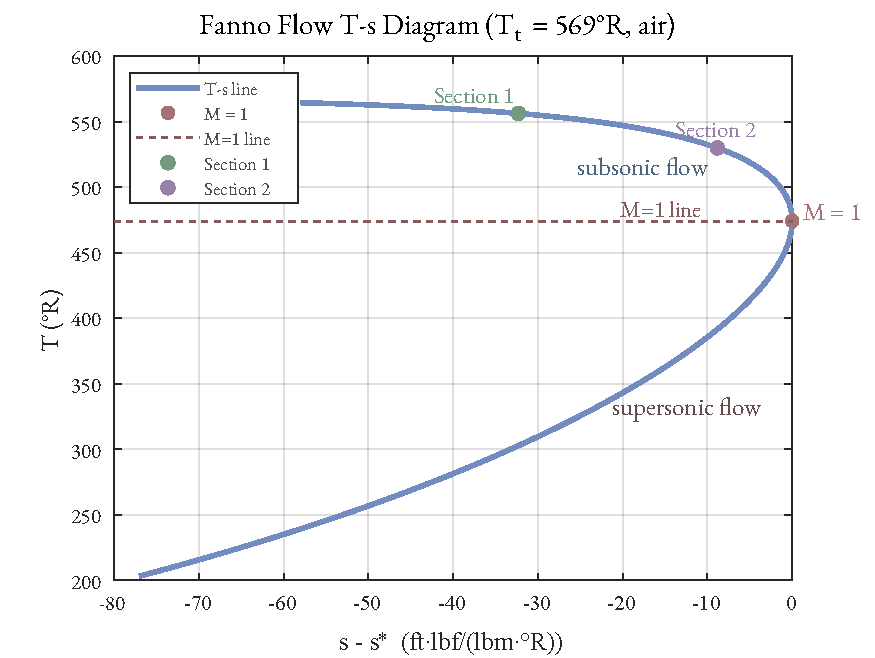
\includegraphics[width=0.8\textwidth]{pic/A5.5.png}
\end{figure}
\end{answerbox}

\question{5.7}{Carbon monoxide flows through an adiabatic system. $M_1 = 4.0$ and $p_{t1} = 45$\,\si{psia}. At a point downstream, $M_2 = 1.8$ and $p_2 = 7.0$\,\si{psia}.\\
(a)	Are there losses in this system? If so, compute $\Delta s$.\\
(b)	Determine the ratio of $A_2/A_1$.
}

\begin{answerbox}
(a) $p_{t2}=p_2\left(1+\dfrac{\gamma -1}{2}M_2^2\right)^{\frac{\gamma}{\gamma -1}}=40.22$\,\si{psia}.

So $e^{-\Delta s/R}=\dfrac{p_{t2}}{p_{t1}}=0.894$.

Thus $\Delta s=-\dfrac{\ln(0.894)\cdot 53.3}{778.2}=0.00794$\,\si{Btu/(lbm-\Rankine)}.

(b) $\dfrac{A_2}{A_1}=\dfrac{M_1}{M_2}\left(\dfrac{1+[(\gamma -1)/2]M_2^2}{1+[(\gamma -1)/2]M_1^2}\right)^{\frac{\gamma+1}{2(\gamma -1)}}e^{\Delta s/R}=0.1502$.
\end{answerbox}

\question{5.9}{Starting with the flow rate as from equation (2.30), derive the following relation:\\
\begin{align*}
  \dfrac{\dot{m}}{A} = M\left(1+[(\gamma -1)/2]M^2\right)^{-(\gamma +1)/2(\gamma -1)}\left(\dfrac{\gamma g_c}{R}\right)^{1/2}\dfrac{p_t}{\sqrt{T_t}}
\end{align*}
}

\begin{answerbox}
From continutiy equation, we have: $\dot{m}=\rho AV=\text{const}$.

So: 
\begin{align*}
  \dfrac{\dot{m}}{A} &=\rho V =\dfrac{p}{RT}M\sqrt{\gamma g_c RT}=pM\sqrt{\frac{\gamma g_c}{RT}}\\
  &=\dfrac{p_t}{\left(1+\frac{\gamma-1}{2}M^2\right)^{\frac{\gamma}{\gamma -1}}}M\sqrt{\frac{\gamma g_c}{R}}\dfrac{\left(1+\frac{\gamma -1}{2}M^2\right)^{\frac{1}{2}}}{\sqrt{T_t}}\\
  &=\left(1+\dfrac{\gamma -1}{2}M^2\right)^{\frac{\gamma +1}{2(1-\gamma)}}M\sqrt{\frac{\gamma g_c}{R}}\dfrac{p_t}{\sqrt{T_t}}\\
  &=M\left(1+[(\gamma -1)/2]M^2\right)^{-(\gamma +1)/2(\gamma -1)}\left(\dfrac{\gamma g_c}{R}\right)^{1/2}\dfrac{p_t}{\sqrt{T_t}}
\end{align*}
\end{answerbox}

\question{5.16}{A converging–diverging nozzle (Figure P5.16) discharges air into a receiver where the static pressure is $15$\,\si{psia}. A\,\si{1-ft^2} duct feeds the nozzle with air at $100$\,\si{psia}, $800$\,\si{\Rankine}, and a velocity such that the Mach number $M_1=0.3$. 
The exit area is such that the pressure at the nozzle exit exactly matches the receiver pressure. Assume steady, one-dimensional flow, perfect gas, and so on. The nozzle is adiabatic and there are no losses.\\
(a)	Calculate the flow rate.\\
(b)	Determine the throat area.\\
(c)	Calculate the exit area.
\begin{figure}[H]
  \centering
  \includegraphics[width=0.5\textwidth]{pic/P5.16.png}
  \caption{Figure P5.16}
\end{figure}
}

\begin{answerbox}
(a) $T_{t1}=T_1\left(1+\dfrac{\gamma-1}{2}M_1^2\right)=814.4$\,\si{\Rankine}.

$p_{t1}=p_1\left(1+\dfrac{\gamma-1}{2}M_1^2\right)^{\frac{\gamma}{\gamma -1}}=106.4$\,\si{psia}.

$\dot{m}=A_1M_1\left(1+[(\gamma -1)/2]M_1^2\right)^{-(\gamma +1)/2(\gamma -1)}\left(\dfrac{\gamma g_c}{R}\right)^{1/2}\dfrac{p_{t1}}{\sqrt{T_{t1}}}=140.4$\,\si{lbm/sec}.

(b) $M_2=1$, and there are no losses, so $\Delta s=0$.

So $A_2=A_1\dfrac{M_1}{M_2}\left(\dfrac{1+[(\gamma -1)/2]M_2^2}{1+[(\gamma -1)/2]M_1^2}\right)^{\frac{\gamma+1}{2(\gamma -1)}}=0.491$\,\si{ft^2}.

(c) There are no losses, so $p_{t1}=p_{t2}$.

Thus $\dfrac{p_{\text{rec}}}{p_{t2}}=\dfrac{p_{\text{rec}}}{p_{t1}}=0.1410$, so $M_3=1.937$.

So $A_3=A_2\dfrac{M_2}{M_3}\left(\dfrac{1+[(\gamma -1)/2]M_3^2}{1+[(\gamma -1)/2]M_2^2}\right)^{\frac{\gamma+1}{2(\gamma -1)}}=0.787$\,\si{ft^2}.
\end{answerbox}

\question{5.19}{Air enters a converging–diverging nozzle with $T_1=22$\,\si{\celsius}, $p_1=10$\,\si{bar} abs., and $V_1\approx 0$. The exit Mach number is $2.0$, the exit area is $0.25$\,\si{m^2}, and the nozzle efficiency is $0.95$.\\
(a)	What are the actual exit values of $T$, $p$, and $p_t$?\\
(b)	What is the ideal exit Mach number?\\
(c)	Assume that all the losses occur in the diverging portion of the nozzle and compute the throat area.\\
(d)	What is the mass flow rate?
}

\begin{answerbox}
(a) In a nozzle, $h_{t1}=h_{t2}$, so that $T_{t1}=T_{t2s}=T_{t2}=295$\,\si{K}.

$T_2=\dfrac{T_{t2}}{1+\frac{\gamma -1}{2}M_2^2}=163.9$\,\si{K}.

And $\eta_n=\dfrac{T1-T2}{T_1-T_{2s}}=0.95$, so $T_{2s}=157.1K$.

So $M_{2s}=2.1$, so $\dfrac{p_{2s}}{p_{t2s}}=0.11$

Thus $p_2=p_{2s}=\dfrac{p_{2s}}{p_{t2s}}\dfrac{p_{t2s}}{p_{t1}}\dfrac{p_{t1}}{p_{1}}p_1=1.1$\,\si{bar}.

$p_{t2}=p_2\left(1+\dfrac{\gamma -1}{2}M_2^2\right)^{\frac{\gamma}{\gamma -1}}=8.61$\,\si{bar}.

(b) $M_{2s}=2.1$

(c) $e^{-\Delta s/R}=\dfrac{p_{t2}}{p_{t1}}=0.861$. $M^{*}=1$.

$\dfrac{A_2}{A^{*}}=\dfrac{M^{*}}{M_2}\left(\dfrac{1+[(\gamma -1)/2]M_2^2}{1+[(\gamma -1)/2]M^{*2}}\right)^{\frac{\gamma+1}{2(\gamma -1)}}e^{\Delta s/R}=1.96$.

$A^{*}=0.1276$\,\si{m^2}.

(d) $\dot{m} = A_2M_2\left(1+[(\gamma -1)/2]M_2^2\right)^{-(\gamma +1)/2(\gamma -1)}\left(\dfrac{\gamma g_c}{R}\right)^{1/2}\dfrac{p_{t2}}{\sqrt{T_{t2}}}=300$\,\si{kg/s}.

\end{answerbox}

\question{5.23}{Assume that a supersonic nozzle operating isentropically delivers air at an exit Mach number of $2.8$. The entrance conditions are $180$\,\si{psia}, $1000$\,\si{\Rankine}, and near-zero Mach number.\\
(a)	Find the area ratio $A_3/A_2$ and the mass flow rate per unit throat area.\\
(b)	What are the receiver pressure and temperature?\\
(c)	If the entire diverging portion of the nozzle were suddenly to detach, what would the Mach number and $\dot{m}/A$ be at the new outlet?
}

\begin{answerbox}
(a) At throat, $M_2=1$, at exit $M_3=2.8$. And as there are no lossed.

So $\dfrac{A_3}{A_2}=\dfrac{M_2}{M_3}\left(\dfrac{1+[(\gamma -1)/2]M_3^2}{1+[(\gamma -1)/2]M_2^2}\right)^{\frac{\gamma+1}{2(\gamma -1)}}=3.5$.

$p_t=180$\,\si{psia}, $T_t=1000$\,\si{\Rankine}.

Thus $\dfrac{\dot{m}}{A_2} = M_2\left(1+\dfrac{\gamma -1}{2}M_2^2\right)^{-(\gamma +1)/2(\gamma -1)}\left(\dfrac{\gamma g_c}{R}\right)^{1/2}\dfrac{p_t}{\sqrt{T_t}}=436$\,\si{lbm/(sec\cdot ft^2)}.

(b) $T_3=T_t\left(1+\dfrac{\gamma -1}{2}M_3^2\right)^{-1}=389.4\,\si{\Rankine}\geqslant T_{\text{rec}}$.

$p_{t1}=p_1\left(1+\dfrac{\gamma-1}{2}M_1^2\right)^{\frac{\gamma}{\gamma -1}}=6.63\,\si{psia}\geqslant p_{\text{rec}}$.

(c) Same.
\end{answerbox}

\newpage

\section{Chapter 6}
\question{6.1}{A standing normal shock occurs in air that is flowing at a Mach number of $1.8$.\\
(a)	What are the pressure, temperature, and density ratios across the shock?\\
(b)	Compute the entropy change for the air as it passes through the shock.\\
(c)	Repeat part (b) for flows at $M = 2.8$ and $3.8$.
}

\begin{answerbox}
(a) $M=1.8$, check the table we gain:

$\dfrac{p_2}{p_1}=3.61, \dfrac{T_2}{T_1}=1.53$.

And $p=\rho RT$, thus $\dfrac{\rho_2}{\rho_1}=\dfrac{p_2/T_2}{p_1/T_1}=2.36$.

(b) $\dfrac{p_{t2}}{p_{t1}}=0.81268=e^{-\Delta s/r}$, so $\Delta s=-\dfrac{\ln(0.81268)\cdot 53.3}{778.2}=0.01421$\,\si{Btu/(lbm-\Rankine)}.

(c) As $M=2.8$, $p_{t2}/p_{t1}=0.38946$, so $\Delta s=-\dfrac{\ln(0.38946)\cdot 53.3}{778.2}=0.06459$\,\si{Btu/(lbm-\Rankine)}.

As $M=3.8$, $p_{t2}/p_{t1}=0.16447$, so $\Delta s=-\dfrac{\ln(0.16447)\cdot 53.3}{778.2}=0.1237$\,\si{Btu/(lbm-\Rankine)}.
\end{answerbox}

\question{6.2}{The difference between the total and static pressure before a shock is $75$\,\si{psi}. What is the maximum static pressure that can exist at this point ahead of the shock? The gas is oxygen. (\textit{Hint:} Start by finding the static and total pressures ahead of the shock for the limiting case of $M = 1.0$.)
}

\begin{answerbox}
$p_t-p=p\left(1+\dfrac{\gamma -1}{2}M^2\right)^{\frac{\gamma}{\gamma-1}}-p=75$.

So $p=\dfrac{75}{\left(1+\frac{\gamma-1}{2}M^2\right)^{\frac{\gamma}{\gamma -1}}-1}=\dfrac{75}{\left(1+0.2M^2\right)^{3.5}-1}$.

There is a shock wave, so $M>1$, thus $p_{\max}=84.0$\,\si{psi}, when $M=1$.
\end{answerbox}

\question{6.3}{In an arbitrary perfect gas, the Mach number before a shock is infinite.\\
(a)	Determine a general expression for the Mach number after the shock. What is the value of this expression for $\gamma = 1.4$?\\
(b)	Determine general expressions for the ratios $p_2/p_1$, $T_2/T_1$, $\rho_2/\rho_1$, and $p_{t2}/p_{t1}$. Do these agree with the values shown in Appendix H for $\gamma = 1.4$?
}

\begin{answerbox}
(a) $M_2^2=\dfrac{M_1^2+2/(\gamma -1)}{[2\gamma /(\gamma -1)]M_1^2-1}$.

As $M_1\to \infty$, thus $\displaystyle M_2=\lim_{M_1\to \infty}\sqrt{\dfrac{M_1^2+2/(\gamma -1)}{[2\gamma /(\gamma -1)]M_1^2-1}}=\sqrt{\dfrac{\gamma -1}{2\gamma}}$.

When $\gamma =1.4$, $M_2=0.378$.

(b) As $M_1\to \infty$, so that:
\begin{align*}
p_2/p_1 &=\lim_{M_1\to \infty}\dfrac{2\gamma}{\gamma +1}M_1^2-\dfrac{\gamma -1}{\gamma +1}=\lim_{M_1\to \infty}\dfrac{2\gamma}{\gamma +1}M_1^2\to \infty\\
T_2/T_1&=\lim_{M_1\to \infty}\dfrac{\{1+[(\gamma -1)/2]M_1^2\}\{[2\gamma /(\gamma -1)]M_1^2-1\}}{[(\gamma+1)^2/2(\gamma -1)]M_1^2}\\
&=\lim_{M_1\to \infty}\dfrac{2\gamma (\gamma -1)}{(\gamma+1)^2}M_1^2\to \infty\\
p_{t2}/p_{t1}&=\lim_{M_1\to \infty}\left(\dfrac{[(\gamma+1)/2]M_1^2}{1+[(\gamma -1)/2]M_1^2}\right)^{\gamma / (\gamma -1)}\left[\dfrac{2\gamma}{\gamma +1}M_1^2-\dfrac{\gamma-1}{\gamma +1}\right]^{1/(1-\gamma)}\\
&=\lim_{M_1\to \infty}\left(\dfrac{\gamma+1}{\gamma-1}\right)^{\gamma/(\gamma-1)}\left[\dfrac{2\gamma}{\gamma+1}M_1^2\right]^{1/(1-\gamma)}\to 0\\
\rho_2/\rho_1&=\lim_{M_1\to \infty}\dfrac{(\gamma+1)M_1^2}{(\gamma -1)M_1^2+2}=\dfrac{\gamma +1}{\gamma -1}
\end{align*}

When $\gamma =1.4$, we have $p_2/p_1=\infty$, $T_2/T_1=\infty$, $p_{t2}/p_{t1}=0$ and $\rho_2/\rho_1=6$.

Agree with.
\end{answerbox}

\question{6.4}{It is known that sonic velocity exists in each throat of the system shown in Figure P6.4. The entropy change for the air is $0.062$\,\si{Btu/lbm-\Rankine}. Negligible friction exists in the duct. Determine the area ratios $A_3/A_1$ and $A_2/A_1$.
\begin{figure}[H]
  \centering
  \includegraphics[width=0.5\textwidth]{pic/P6.4.png}
  \caption{Figure P6.4}
\end{figure}
}

\begin{answerbox}
As $M_1=M_3=1$ and negligible friction, so $A_1=A_2^{*}$, $A_3=A_{2\prime}^{*}$.

Thus $\dfrac{A_3}{A_1}=\dfrac{A_{2\prime}^{*}}{A_2^{*}}=e^{\Delta s/R}=2.472$.

And $\dfrac{p_{t2\prime}}{p_{t2}}=e^{-\Delta s/R}=0.4048$.

Check the table we gain $M_2=2.75, M_{2\prime}=0.49$.

So $\dfrac{A_2}{A_1}=3.35$.
\end{answerbox}

\question{6.5}{Air flows in the system shown in Figure P6.5. It is known that the Mach number after the shock is $M_3=0.52$. Considering $p_1$ and $p_2$, it is also known that one of these pressures is twice the other.\\
(a)	Compute the Mach number at section 1.\\
(b)	What is the area ratio $A_1/A_2$?
\begin{figure}[H]
  \centering
  \includegraphics[width=0.5\textwidth]{pic/P6.5.png}
  \caption{Figure P6.5}
\end{figure}
}

\begin{answerbox}
(a) Check the table we gain $M_2=2.43$, or you can use $M_2=\sqrt{\dfrac{M_3^2+2/(\gamma -1)}{[2\gamma /(\gamma -1)]M_3^2-1}}$, also can gain $M_2=2.43$.

$p_1<p_2$, so $p_2=2p_1$.

Thus $\dfrac{p_2}{p_1}=\left(\dfrac{1+[(\gamma -1)/2]M_1^2}{1+[(\gamma-1)/2]M_2^2}\right)^{\gamma/(\gamma-1)}=2$, so $M_1=2.88$.

(b) Check the table: $\dfrac{A_1}{A_1^{*}}=3.77711$, $\dfrac{A_2}{A_2^{*}}=2.47061$.

So $\dfrac{A_1}{A_2}=\dfrac{A_1}{A_1^{*}}\dfrac{A_1^{*}}{A_2^{*}}\dfrac{A_2^{*}}{A_2}=1.53$.
\end{answerbox}


\question{6.11}{The diverging section of a supersonic nozzle is formed from the frustrum of a cone. When operating at its third critical point with nitrogen, the exit Mach number is $2.6$. Compute the operating pressure ratio that will locate a normal shock as shown in Figure P6.11.
\begin{figure}[H]
  \centering
  \includegraphics[width=0.5\textwidth]{pic/P6.11.png}
  \caption{Figure P6.11}
\end{figure}
}

\begin{answerbox}
Let the throat area be $A_1$, the exit area $A_e$, and the areas just
upstream and downstream of the normal shock be $A_2$ and $A_3$.
For a conical frustum, the area varies linearly from $A_1$ to $A_e$.
With the shock located at $3/4$ of the diverging length,

\[
A_2 = A_1 + 0.75\,(A_e - A_1),
\Rightarrow 
\frac{A_2}{A_1}
=1+0.75\left(\frac{A_e}{A_1}-1\right).
\]

When operating at its third critical point with nitrogen, the exit Mach number is $2.6$

So $\dfrac{A_e}{A_1}=\dfrac{A_e}{A_e^{*}}=2.89598$

So $\dfrac{A_2}{A_1}=2.422$.


From the isentropic area-Mach relation, $M_2=2.41$.


Across the normal shock, $M_3=0.52$.

Subsonic isentropic flow to the exit gives $\dfrac{A_e}{A_e^{*\prime}}=\dfrac{A_e}{A_3}\dfrac{A_3}{A_3^{*}}\dfrac{A_3^{*}}{A_e^{*\prime}}=1.558$.

Thus $M_4=0.41$.

And $p_{t4}A_4^{*}=p_{t1}A_1^{*}$.

Thus $\dfrac{p_{4}}{p_{t1}} = \dfrac{p_{4}}{p_{t4}}\dfrac{p_{t4}A_{1}^{*}}{p_{t1}A_{4}^{*}}\dfrac{A_{4}}{A_{4}^{*}} = 0.498$

\end{answerbox}

\newpage

\section{Chapter 7}

\question{7.4}{Oxygen at 100\,\si{\Fahrenheit} and 20 \,\si{psia} is flowing at 450 \,\si{ft/sec} in a duct. A valve is quickly shut,
causing a normal shock to travel back through the duct.\\
(a) Determine the speed of the traveling shock wave.\\
(b) What are the temperature and pressure of the oxygen that is brought to rest?
}

\begin{answerbox}
$\Delta V=450$\,\si{ft/sec}, and \(a_1{\prime}=\sqrt{\gamma g_c R T_1^{\prime}}=1103.90\)\,\si{ft/sec}.

Thus \(\dfrac{\Delta V}{a_1^{\prime}}=0.4076\), check the table \(M_1^{\prime}=1.27, M_2^{\prime}=0.80164, \dfrac{T_2^{\prime}}{T_1^{\prime}}=1.97175, \dfrac{p_2^{\prime}}{p_1^{\prime}}=1.71505\).

(a) \(V_S=V_2^{\prime}=M_2^{\prime}a_2^{\prime}\).

\(T_2^{\prime}=655.91\)\,\si{\Rankine}.

So \(a_2^{\prime}=\sqrt{\gamma g_c R T_2^{\prime}}=1195.05\)\,\si{ft/sec}.

\(\therefore V_S=M_2^{\prime}a_2^{\prime}=985\)\,\si{ft/sec}.

(b) \(T_2=T_2^{\prime}=655.91\,\si{\Rankine}, p_2=p_2^{\prime}=34.30\,\si{psia}\).
\end{answerbox}

\question{7.5}{A closed tube contains nitrogen at $20$\,\si{\celsius} and a pressure of $1 \times 10^4$\,\si{N/m^2} (Figure P7.5).
A shock wave progresses through the tube at a speed of $380$\,\si{m/s}.\\
(a) Calculate the conditions that exist immediately after the shock wave passes a given point. (The fact that this is inside a tube should not bother you, as it is merely a normal shock moving into a gas at rest.)\\
(b) When the shock wave hits the end wall, it is reflected back. What are the temperature and pressure of the gas between the wall and the reflected shock? At what speed is the reflected shock traveling? (This is just like the sudden closing of a valve in a duct.)
\begin{figure}[H]
  \centering
  \includegraphics[width=0.5\textwidth]{pic/P7.5.png}
  \caption{Figure P7.5}
\end{figure}
}

\begin{answerbox}
(a) $V_1^{\prime}=V_S=380\,\si{m/s}, p_1^{\prime}=1\times 10^4\,\si{N/m^2}, T_{1^{\prime}=20+273=293\,\si{K}, V_2^{\prime}=V_S-V_2}$.

So $a_1^{\prime}=\sqrt{\gamma g_c R T_1^{\prime}}=348\,\si{m/s}$, thus $M_1^{\prime}=1.09$.

Check the table, $M_2^{\prime}=0.91965, \dfrac{p_2^{\prime}}{p_1^{\prime}}=1.21945, \dfrac{T_2^{\prime}}{T_1^{\prime}}=1.05856$.

So $T_2=T_2^{\prime}=310\,\si{K}, p_2=p_2^{\prime}=1.219\times 10^4\,\si{N/m^2}$.

Thus $a_2^{\prime}=\sqrt{\gamma g_c R T_2^{\prime}}=358\,\si{m/s}$, so $V_2^{\prime}=329.6\,\si{m/s}$.

So $V_2=V_S-V_2^{\prime}=50.3$\,\si{m/s}.

(b) $\Delta V=50.3\,\si{m/s}$, and $a_2^{\prime}=358$\,\si{m/s}.

Thus $\dfrac{\Delta V}{a_2^{\prime}}=0.1405$. Check the table $M_2^{\prime}=1.09, M_3^{\prime}=0.91965, \\ \dfrac{p_3^{\prime}}{p_2^{\prime}}=1.21945, \dfrac{T_3^{\prime}}{T_2^{\prime}}=1.05856$

So $p_3=p_3^{\prime}=1.48\times 10^4\,si{N/m^2}, T_3=T_3^{\prime}=328\,\si{K}$.

Thus $a_3^{\prime}=\sqrt{\gamma g_c R T_3^{\prime}}=368\,\si{m/s}$.

So $V_S=V_3^{\prime}=M_3^{\prime}a_3^{\prime}=340\,\si{m/s}$.
\end{answerbox}

\question{7.6}{An oblique shock forms in air at an angle of $\theta = \ang{30}$. Before passing through the shock, the air has a temperature of $60$\,\si{\Fahrenheit}, a pressure of $10$\,\si{psia}, and is traveling at $M = 2.6$.\\
(a) Compute the normal and tangential velocity components before and after the shock.\\
(b) Determine the temperature and pressure after the shock.\\
(c) What is the deflection angle?
}

\begin{answerbox}
(a) $a_1=\sqrt{\gamma g_c R T_1}=1117.43\,\si{ft/sec}$.

So before the shock $V_{1n}=M_1a_1\sin\theta=1452.66\,\si{ft/sec}, \\V_{1t}=M_1a_1\cos\theta=2516.07\,\si{ft/sec}, M_{1n}=M_1\sin\theta=1.3$.

Check the table: $M_{2n}=0.78596, \dfrac{\Delta V}{a_1}=0.44231, \dfrac{T_2}{T_1}=1.19087, \dfrac{p_2}{p_1}=1.80500$.

So after the shock $V_{2n}=958.41\,\si{ft/sec}, V_{2t}=V_{1t}=2516.07\,\si{ft/sec}$.

(b) $T_2=618.86\,\si{\Rankine}, p_2=18.05\,\si{psia}$.

(c) $\beta=\arctan\dfrac{V_{2t}}{V_{2n}}=\ang{69.1}$.

So $\delta =\beta+\theta-\ang{90}=\ang{9.1}$.
\end{answerbox}

\question{7.8}{Air at $800\,\si{\Rankine}$ and $15$\,\si{psia} is flowing at a Mach number of $M = 1.8$ and is deflected through a \ang{15} angle. The directional change is accompanied by an oblique shock.\\
(a) What are the possible shock angles?\\
(b) For each shock angle, compute the temperature and pressure after the shock.
}

\begin{answerbox}
(a) Check the chart: $\theta=\ang{52}~\text{or}~\ang{77}$.

(b) When $\theta=\ang{77}$, it's a strong shock. $M_{1n}=M_1\sin\theta=1.753$.

So $\dfrac{p_2}{p_1}=1+\dfrac{2\gamma}{\gamma+1}\left(M_{1n}^2-1\right)=3.422, \dfrac{T_2}{T_1}=\dfrac{p_2}{p_1}\dfrac{2+(\gamma-1)M_{1n}^2}{(\gamma+1)M_{1n}^2}=1.497$.

Thus $p_2=51.3$\,\si{psia}, $T_2=1198$\,\si{\Rankine}.

When $\theta=\ang{52}$, it's a weak shock. $M_{1n}=M_1\sin\theta=1.418$.

So $\dfrac{p_2}{p_1}=1+\dfrac{2\gamma}{\gamma+1}\left(M_{1n}^2-1\right)=2.181, \dfrac{T_2}{T_1}=\dfrac{p_2}{p_1}\dfrac{2+(\gamma-1)M_{1n}^2}{(\gamma+1)M_{1n}^2}=1.267$.

Thus $p_2=32.7$\,\si{psia}, $T_2=1013$\,\si{\Rankine}.
\end{answerbox}

\question{7.11}{A pitot tube is installed in a wind tunnel in the manner shown in Figure 7.13. The tunnel air temperature is $500$\,\si{\Rankine} and the static tap ($p_1$) indicates a pressure of $14.5$\,\si{psia}.\\
(a) Determine the tunnel air velocity if the stagnation probe ($p_{t2}$) indicates $65$\,\si{psia}.\\
(b) Suppose that $p_{t2} = 26$\,\si{psia}. What is the tunnel velocity under this condition?
\begin{figure}[H]
  \centering
  \includegraphics[width=0.3\textwidth]{pic/P7.11.png}
  \caption{Figure 7.13}
\end{figure}
}

\begin{answerbox}
(a) Assume it is subsonic flow, Thus $p_{t2}=p_{t1}=p_1\left(1+\dfrac{\gamma-1}{2}M_1^2\right)^{\frac{\gamma}{\gamma-1}}$.

Obtain $M_1=1.64>1$, so it's supersonic flow.

And $\dfrac{p_{t2}}{p_1}=4.483$, so $M_1=1.76$.

and $a_1=\sqrt{\gamma g_c R T}=1096\,\si{ft/sec}$, so $V_1=M_1a_1=1928$\,\si{ft/sec}.

(b) Assume it is subsonic flow, Thus $p_{t2}=p_{t1}=p_1\left(1+\dfrac{\gamma-1}{2}M_1^2\right)^{\frac{\gamma}{\gamma-1}}$.

Obtain $M_1=0.953$, so $V_1=M_1a_1=1044.3$\,\si{ft/sec}.
\end{answerbox}

\question{7.13}{Pictured in Figure P7.13 is the air inlet to a jet aircraft. The plane is operating at $50,000$\,\si{ft}, where the the pressure is $243$\,\si{psfa} and the temperature is $392$\,\si{\Rankine}. Assume that the flight speed is $M_0 = 2.5$.\\
(a) What are the conditions of the air (temperature, pressure, and entropy change) just after it passes through the normal shock?\\
(b) Draw a reasonably detailed T –s diagram for the air inlet. Start the diagram at the free stream and end it at the subsonic diffuser entrance to the compressor.\\
(c) If the single \ang{15} wedge is replaced by a double wedge of \ang{7} and \ang{8} (see Figure 7.15), determine the conditions of the air after it enters the diffuser.\\
(d) Compare the losses for parts (a) and (c).
\begin{figure}[H]
  \centering
  \includegraphics[width=0.5\textwidth]{pic/P7.13.png}
  \caption{Figure P7.13}
\end{figure}
}

\begin{answerbox}
(a) $M_0=2.5$, $\delta=\ang{15}$ and it's weak shock.

So $\theta=\ang{36.94}$, $M_1=1.874$.

$\dfrac{p_1}{p_0}=2.468, \dfrac{p_{t1}}{p_{t0}}=0.929, \dfrac{T_1}{T_0}=1.322$.

So $p_1=599.7$\,\si{psfa}, $T_1=518.2$\,\si{\Rankine}.

After the normal shock, $M_2=0.6$

$\dfrac{p_2}{p_1}=3.93, \dfrac{p_{t2}}{p_{t1}}=0.78, \dfrac{T_2}{T_1}=1.587$.

So $p_2=2356.8$\,\si{psfa}, $T_2=822.4$\,\si{\Rankine}.

And $\dfrac{p_{t2}}{p_{t0}}=e^{-\Delta s/R}$, thus $\Delta s=0.0221$\,\si{Btu/(lbm\text{-}\Rankine)}.

(b) Use Matlab to draw the diagram.
\begin{figure}[H]
  \centering
  \includegraphics[width=0.8\textwidth]{pic/A7.13.png}
\end{figure}

(c) $M_0=2.5$, $\delta_1=\ang{7}$ and it's weak shock.

So $\theta=\ang{29.1}$, $M_1=2.21$.

$\dfrac{p_1}{p_0}=1.56, \dfrac{p_{t1}}{p_{t0}}=0.991, \dfrac{T_1}{T_0}=1.138$.

$M_1=2.21$, $\delta_2=\ang{8}$ and it's weak shock.

So $\theta=\ang{33.67}$, $M_2=1.91$.

$\dfrac{p_2}{p_1}=1.585, \dfrac{p_{t2}}{p_{t1}}=0.99, \dfrac{T_2}{T_1}=1.144$.

After the normal shock, $M_3=0.59$

$\dfrac{p_2}{p_1}=4.089, \dfrac{p_{t2}}{p_{t1}}=0.763, \dfrac{T_2}{T_1}=1.616$.

So $p_3=2465.2$\,\si{psfa}, $T_3=825.7$\,\si{\Rankine}.

And $\dfrac{p_{t3}}{p_{t0}}=e^{-\Delta s^{\prime}/R}$, thus $\Delta s^{\prime}=0.0198$\,\si{Btu/(lbm\text{-}\Rankine)}.

(d) $\Delta s>\Delta s^{\prime}$, so (c) losses are smaller.

\end{answerbox}

\question{7.15}{For the flow situation shown in Figure P7.15, $M_1 = 1.8$, $T_1 = 600$\,\si{\Rankine}, $p_1 = 15$\,\si{psia}, and $\gamma = 1.4$.\\
(a) Find conditions in region 2 assuming that they are supersonic.\\
(b) What must occur along the dashed line?\\
(c) Find the conditions in region 3.\\
(d) Find the value of $T_2$, $p_2$, and $M_2$ if $p_{t2} = 71$\,\si{psia}.\\
(e) How would the problem change if the flow in region 2 were subsonic?
\begin{figure}[H]
  \centering
  \includegraphics[width=0.5\textwidth]{pic/P7.15.png}
  \caption{Figure P7.15}
\end{figure}
}

\begin{answerbox}
(a) For $M_1=1.8$, $\delta_1=\ang{10}$ and it's a weak shock, so $\theta_1=\ang{44}$.

So $M_{1n}=1.25$, check the table $M_{2n}=0.812$.

So $M_2=\dfrac{M_{2n}}{\sin(\theta_1-\delta_1)}=1.45$. $\dfrac{p_2}{p_1}=1.66$, $\dfrac{T_2}{T_1}=1.16$.

Thus $p_2=24.9$\,\si{psia}, $T_2=696$\,\si{\Rankine}.

(b) Oblique shock with $\delta_2=\ang{10}$.

(c) For $\delta_2=\ang{10}$, $M_2=1.45$, and it's a weak shock, so $\theta_2=\ang{61}$.

So $M_{2n}=1.25$ check the table $M_{3n}=0.81$.

So $M_3=\dfrac{M_{3n}}{\sin(\theta_2-\delta_2)}=1.03$, $\dfrac{p_3}{p_2}=1.71$, $\dfrac{T_3}{T_2}=1.17$.

Thus $p_3=42.6$\,\si{psia}, $T_3=814.3$\,\si{\Rankine}.

(d) $p_{t1}=p_1\left(1+\dfrac{\gamma-1}{2}M_1^2\right)^{\frac{\gamma}{\gamma-1}}=86.2$\,\si{psia}.

So $\dfrac{p_{t2}}{p_{t1}}=0.823$, thus it's a strong shock.

Thus $M_2=0.7$, $\dfrac{p_2}{p_1}=3.54$, $\dfrac{T_2}{T_1}=1.51$.

Thus $p_2=53.1$\,\si{psia}, $T_2=906$\,\si{\Rankine}.

(e) There are no shocks after downstream.
\end{answerbox}

\question{7.16}{Carbon monoxide flows in the duct shown in Figure P7.16. The first shock, which turns the flow \ang{15}, is observed to form at a \ang{40} angle. The flow is known to be supersonic in regions 1 and 2 and subsonic in region 3.\\
(a) Determine $M_3$ and $\beta$.\\
(b) Determine the pressure ratios $p_3/p_1$ and $p_{t3}/p_{t1}$.
\begin{figure}[H]
  \centering
  \includegraphics[width=0.5\textwidth]{pic/P7.16.png}
  \caption{Figure P7.16}
\end{figure}
}

\begin{answerbox}
(a) For $\gamma=1.4$, $\theta_1=\ang{40}$, $\delta_1=\ang{15}$, $\tan\delta_1=\cot\theta_1\left(\dfrac{M_1^2\sin^2\theta_1-1}{M_1^2(\gamma+\cos2\theta_1)+2}\right)$.

Thus $M_1=2.29$, so $M_2=1.69$.

So $\dfrac{p_{t2}}{p_{t1}}=0.941$, $\dfrac{p_2}{p_1}=2.33$.

And because $\delta_2=\ang{15}$, $M_3<1$, thus it's a strong shock.

So $\delta_2=\ang{73}$, $M_3=0.783$.

So $\beta=\theta_2-\delta_2=\ang{58}$.

(b) Check the table, $\dfrac{p_3}{p_2}=2.89$, $\dfrac{p_{t3}}{p_{t2}}=0.89$.

Thus $\dfrac{p_3}{p_1}=6.72$, $\dfrac{p_{t3}}{p_{t1}}=0.837$.
\end{answerbox}

\question{7.17}{A uniform flow of air has a Mach number of $3.3$. The bottom of the duct is bent upward at a \ang{25} angle. At the point where the shock intersects the upper wall, the boundary is bent \ang{5} upward as shown in Figure P7.17. Assume that the flow is supersonic throughout the system. Compute $M_3$, $p_3/p_1$, $T_3/T_1$, and $\beta$.
\begin{figure}[H]
  \centering
  \includegraphics[width=0.5\textwidth]{pic/P7.17.png}
  \caption{Figure P7.17}
\end{figure}
}

\begin{answerbox}
For $\delta_1=\ang{25}$, $M_1=3.3$, $M_2>1$, so it's a weak shock.

Thus $\theta_1=\ang{41.9}$, so $M_{1n}=2.2$, $M_{2n}=0.55$.

So $M_2=1.88$ $\dfrac{p_2}{p_1}=5.494$, $\dfrac{T_2}{T_1}=1.859$.

And $\delta_2=\delta_1-\ang{5}=\ang{20}$, so $\theta_2=\ang{59.2}$, $M_3=1.05$.

$\dfrac{p_3}{p_2}=2.88$, $\dfrac{T_3}{T_2}=1.40$.

Thus $\dfrac{p_3}{p_1}=15.82$, $\dfrac{T_3}{T_1}=2.6$.
\end{answerbox}

\newpage

\section{Chapter 8}

\question{8.2}{A Schleiren photo of the flow around a corner reveals the edges of the expansion fan to be indicated by the angles shown in Figure P8.2. Assume that $\gamma = 1.4$.\\
(a) Determine the Mach number before and after the corner.\\
(b) Through what angle was the flow turned, and what is the angle of the expansion fan ($\theta_3$)?
\begin{figure}[H]
  \centering
  \includegraphics[width=0.5\textwidth]{pic/P8.2.png}
  \caption{Figure P8.2}
\end{figure}
}

\begin{answerbox}
(a) From Figure P8.2, we gian $\theta_1=\ang{147.2}$, $\theta_2=\ang{19.2}$.

So $\mu_1=\ang{37.3}$, $\mu_2=\ang{19.2}$.

Check the table we obtain: $M_1=1.65$, $M_2=3.04$.

(b) From the table $\nu_1=\ang{16.3}$, $\nu_2=\ang{50.5}$.

Thus $\Delta \nu=\nu_2-\nu_1=\ang{34.2}$.

And $\theta_3=\mu_1-\mu_2+\Delta \nu=\ang{52.3}$.
\end{answerbox}

\question{8.4}{In a problem similar to Problem 8.2, $\theta_1$ is unknown, but $\theta_2 = \ang{15.90}$ and $\theta_3 = \ang{82.25}$. Can you determine the initial Mach number?}

\begin{answerbox}
We have $\mu_2=\theta_2=\ang{15.9}$.

Check the table: $M_2=3.65$, $\nu_2=\ang{60.85}$.

Because $\theta_3=\mu_1-\mu_2+\Delta \nu$, $\Delta \nu=\nu_2-\nu_1$,

$\mu_1=\cot^{-1}(M_1^2-1)^{\frac{1}{2}}$, $\nu_1=\left(\dfrac{\gamma+1}{\gamma-1}\right)^{\frac{1}{2}}\tan^{-1}\left[\dfrac{\gamma-1}{\gamma+1}(M_1^2-1)\right]^{\frac{1}{2}}-\tan^{-1}(M_1^2-1)^{\frac{1}{2}}$.

Thus:
\[
\resizebox{\textwidth}{!}{$
\ang{82.25}=\cot^{-1}(M_1^2-1)^{\frac{1}{2}}-\ang{15.9}+\ang{60.85}-\left\{\left(\dfrac{\gamma+1}{\gamma-1}\right)^{\frac{1}{2}}\tan^{-1}\left[\dfrac{\gamma-1}{\gamma+1}(M_1^2-1)\right]-\tan^{-1}(M_1^2-1)^{\frac{1}{2}}\right\}
$}
\]

So $M_1=1.39$.
\end{answerbox}

\question{8.6}{A smooth concave turn similar to that shown in Figure 8.2 turns the flow through a \ang{30} angle. The fluid is oxygen and it approaches the turn at $M_1 = 4.0$.\\
(a) Compute $M_2$, $T_2/T_1$, and $p_2/p_1$ via the Prandtl–Meyer compression which occurs close to the wall.\\
(b) Compute $M_2^{\prime}$, $\pp{T_2}/T_1$, and $\pp{p_2}/p_1$ via the oblique shock that forms away from the wall. Assume that this flow is also deflected by \ang{30}.\\
(c) Draw a T–s diagram showing each process.\\
(d) Can these two regions coexist next to one another?\\
\begin{figure}[H]
  \centering
  \includegraphics[width=0.5\textwidth]{pic/P8.6.png}
  \caption{Figure 8.2}
\end{figure}
}

\begin{answerbox}
(a) \(M_1=4.0\), Check the table: $\nu_1=\ang{65.78}$, $\dfrac{p_1}{p_{t1}}=0.00659$, $\dfrac{T_1}{T_{t1}}=0.23810$.

Form Figure 8.2 we gain $\Delta \nu=\ang{-30}$, thus $\nu_2=\ang{35.78}$.

Check the table: $M_2=2.36$, $\dfrac{p_2}{p_{t2}}=0.07281$, $\dfrac{T_2}{T_2^{t2}}=0.47305$.

So $p_2/p_1=11.05$, $T_2/T_1=1.987$.

(b) From Figure 8.2 we know $\delta=\ang{30}$.

And $M_1=4.0$, it's a weak shock, Thus $\theta=\ang{45.22}$.

Thus $M_2=1.85$, $\dfrac{p_2}{p_1}=9.243$, $\dfrac{T_2}{T_1}=2.495$.

(c) For (a) it's isentropic flow. 

\begin{figure}[H]
  \centering
  \includegraphics[width=0.8\textwidth]{pic/A8.6_1.png}
\end{figure}

For (b):
\begin{figure}[H]
  \centering
  \includegraphics[width=0.8\textwidth]{pic/A8.6_2.png}
\end{figure}

(d) No.
\end{answerbox}

\question{8.12}{Air flows through a converging–diverging nozzle that has an area ratio of $3.5$. The nozzle is operating at its third critical (design condition). The jet stream strikes a twodimensional wedge with a total wedge angle of \ang{40} as shown in Figure P8.12.\\
(a) Make a sketch to show the initial wave pattern that results from the jet stream striking the wedge.\\
(b) Show the additional wave pattern formed by the interaction of the initial wave system with the free boundary. Mark the flow direction in the region following each wave form and show what happens to the free boundary.\\
(c) Compute the Mach number and direction of flow after the air jet passes through each system of waves.
\begin{figure}[H]
  \centering
  \includegraphics[width=0.5\textwidth]{pic/P8.12.png}
  \caption{Figure P8.12}
\end{figure}
}

\begin{answerbox}
The nozzle is operating at its third critical (design condition), thus $M_1=2.8$, $p_1=p_{\mathrm{amb}}$.

(a) For $\delta=\ang{20}$, thus $\theta=\ang{39.48}$, $M_2=1.86$.
\begin{figure}[H]
  \centering
  \includegraphics[width=0.6\textwidth]{pic/A8.12_1.png}
\end{figure}

(b) After the shock, $p_2=3.53p_1=3.53p_{\mathrm{amb}}$.

When an oblique shock wave encounters a free boundary, a Prandtl-Meyer expansion wave is generated to ensure pressure equilibrium.

Thus $p_3=p_{\mathrm{amb}}$.

Check the table we gain $M_3=2.67$, $\nu_3=\ang{42.7}$.

And $\nu_2=\ang{22.2}$, so $\Delta \nu=\ang{20.5}$.

\begin{figure}[H]
  \centering
  \includegraphics[width=0.6\textwidth]{pic/A8.12_2.png}
\end{figure}

(c) $M_2=1.86$, \ang{20} from centerline.

$M_3=2.67$, \ang{40.5} from centerline.
\end{answerbox}

\question{8.15}{Consider the expression for the Prandtl–Meyer function that is given in equation (8.48).\\
(a) how that the maximum possible value for $\nu$ is
\[
\nu_{\max}=\dfrac{\pi}{2}\left(\sqrt{\dfrac{\gamma+1}{\gamma-1}}-1\right)
\]\\
(b) At what Mach number does this occur?\\
(c) If $\gamma = 1.4$, what are the maximum turning angles for accelerating flows with initial Mach numbers of $1.0$, $2.0$, $5.0$, and $10.0$?\\
(d) If a flow of air at $M = 2.0$, $p = 100$\,\si{psia}, and $T = 600$\,\si{\Rankine} expands through its maximum turning angle, what is the velocity?
}

\begin{answerbox}
$\nu(M)=\left(\dfrac{\gamma+1}{\gamma-1}\right)^{\frac{1}{2}}\tan^{-1}\left[\dfrac{\gamma-1}{\gamma+1}(M^2-1)\right]^{\frac{1}{2}}-\tan^{-1}(M^2-1)^{\frac{1}{2}}$

(a) Differentiating the above equation yields:$\dfrac{\mathrm{d}\nu}{\mathrm{d}M} = \dfrac{\sqrt{M^2-1}}{M \left( 1 + \frac{\gamma-1}{2} M^2 \right)}$.

For $M>1$, we always have: $\dfrac{\mathrm{d}\nu}{\mathrm{d}M}>0$.

Thus This is a monotonically increasing function, and it reaches its maximum value when $M \to \infty$.

So $\displaystyle \nu_{\max}=\lim_{M \to \infty}\left(\dfrac{\gamma+1}{\gamma-1}\right)^{\frac{1}{2}}\tan^{-1}\left[\dfrac{\gamma-1}{\gamma+1}(M^2-1)\right]^{\frac{1}{2}}-\tan^{-1}(M^2-1)^{\frac{1}{2}}=\dfrac{\pi}{2}\left(\sqrt{\dfrac{\gamma+1}{\gamma-1}}-1\right)$.

(b) $M \to \infty$.

(c) $\gamma = 1.4$, so $\nu_{\max}=\ang{130.45}$.

From equation (8.40), we obtain: $\nu_{1.0}=\ang{0}$, $\nu_{2.0}=\ang{26.37}$, $\nu_{5.0}=\ang{76.92}$, $\nu_{10.0}=\ang{102.31}$.

So $\Delta \nu_{1.0}=\ang{130.45}$, $\Delta \nu_{2.0}=\ang{104.08}$, $\Delta \nu_{5.0}=\ang{53.53}$, $\Delta \nu_{10.0}=\ang{28.14}$.

(d) For it's isentropic, $T_t=T_1\left(1+\dfrac{\gamma-1}{2}M_1^2\right)=1080\,\si{\Rankine}=\mathrm{const}$.

When air expands through its maxiumum turning angle, $M_2 = \infty$, thus $T_2\to 0$

So from $h_t=h_2+\dfrac{V_2^2}{2g_c}$ we gain $c_p T_t=c_p T_2+\dfrac{V_2^2}{2g_c}$.

Thus $V_2=\sqrt{2 g_c c_p T_t}=3604$\,\si{ft/sec}.
\end{answerbox}

\question{8.16}{Flow, initially at a Mach number of unity, expands around a corner through angle $\nu$ and reaches Mach number $M_2$ (see Figure P8.16). Lengths $L_1$ and $L_2$ are measured perpendicular to the wall and measure the distance out to the same streamline as shown.\\
(a) Derive an equation for the ratio $L_2/L_1 = f(M2,\gamma)$. (Hints: What fundamental concept must be obeyed? What kind of process is this?)\\
(b) If $M_1 = 1.0$, $M_2 = 1.79$, and $\gamma = 1.67$, compute the ratio $L_2/L_1$.
\begin{figure}[H]
  \centering
  \includegraphics[width=0.5\textwidth]{pic/P8.16.png}
  \caption{Figure P8.16}
\end{figure}
}

\begin{answerbox}
(a) From continuity equation: $\rho_1 V_1 A_1=\rho_2 V_2 A_2$.

For For a two-dimensional flow with a constant depth $b$, $A=bL$.

Thus $\rho_1 V_1 A_1=\rho_2 V_2 A_2 \rightarrow \rho_1 V_1 L_1=\rho_2 V_2 L_2 \Rightarrow \dfrac{L_2}{L_1}=\dfrac{\rho_1 V_1}{\rho_2 V_2}$.

In an isentropic flow: $T=T_t\left(1+\dfrac{\gamma-1}{2}M^2\right)^{-1}$, $\rho = \rho_t \left( 1 + \dfrac{\gamma-1}{2} M^2 \right)^{-\frac{1}{\gamma-1}}$

And $V=Ma=M\sqrt{\gamma g_c R T}$.

So $\rho V=\rho_t \sqrt{\gamma g_c R T_t}M\left(1+\dfrac{\gamma-1}{2}M^2\right)^{-\frac{\gamma+1}{2(\gamma-1)}}$.

So $\dfrac{L_2}{L_1}=\dfrac{M_1\left(1+\frac{\gamma-1}{2}M_1^2\right)^{-\frac{\gamma+1}{2(\gamma-1)}}}{M_2\left(1+\frac{\gamma-1}{2}M_2^2\right)^{-\frac{\gamma+1}{2(\gamma-1)}}}$.

$M=1.0$, thus $\dfrac{L_2}{L_1}=\dfrac{1}{M_2}\left(\dfrac{\gamma+1}{2}\right)^{\frac{\gamma+1}{2(\gamma-1)}}\left(1+\dfrac{\gamma-1}{2}M_2^2\right)^{\frac{\gamma+1}{2(\gamma-1)}}$.

(b) For$M_2=1.79$, $\gamma=1.67$, $\dfrac{L_2}{L_1}=1.343$.
\end{answerbox}

\newpage

\section{Chapter 9}

\question{9.5}{Air flows in an $8$-\si{cm}-inside diameter pipe that is $4$\,\si{m} long. The air enters with a Mach number of $0.45$ and a temperature of $300$\,\si{K}.\\
(a) What friction factor would cause sonic velocity at the exit?\\
(b) If the pipe is made of cast iron, estimate the inlet pressure.
}

\begin{answerbox}
(a) $M_1=0.45$, at exit $M_2=1$.

Check the table $\dfrac{f\Delta x}{D}=\dfrac{fL_{\max 1}}{D}=1.566$.

And $\Delta x=8$\,\si{m}, $D=0.08$\,\si{m}.

Thus $f=0.0313$.

(b) The pipe is made of cast iron, check the table: $\varepsilon=0.00026$\,\si{m}.

Thus $\dfrac{\varepsilon}{D}=0.00323$.

For $f=0.313$, view the Moody diagram we gain: $\ReN=2.2\times 10^4$.

And $\ReN=\dfrac{\rho V D}{\mu}$, $\rho=\dfrac{p}{R T}$, $V=M\sqrt{\gamma R T}$.

So the inlet pressure $p_1=2730$\,\si{Pa}.
\end{answerbox}

\question{9.13}{Ambient air at \SI{60}{\Fahrenheit} and $14.7$ psia accelerates isentropically into a $12$-in.-diameter duct. After $100$\,\si{ft} the duct transitions into an $8 \times 8$ in. square section where the Mach number is $0.50$. Neglect all frictional effects except in the constant-area duct, where $f = 0.04$.\\
(a) Determine the Mach number at the duct entrance.\\
(b) What are the temperature and pressure in the square section?\\
(c) How much $8 \times 8$ in. square duct could be added before the flow chokes? (Assume that $f = 0.04$ in this duct also.)
}

\begin{answerbox}
(a) $M_3=0.50$, Thus $\dfrac{A_3}{A^{*}_3}=1.34$.

The process of the flow contracting into an $8\times 8$ in. square is an isentropic compression, and $\dfrac{A_2}{A_3}=1.77$.

Thus $\dfrac{A_2}{A_2^{*}}=2.37$.

Thus $M_2=0.254$, so $\dfrac{fL_{\max 2}}{D}=8.15$.

And $\dfrac{f\Delta x}{D}=4$, so $\dfrac{fL_{\max 1}}{D}=\dfrac{fL_{\max 2}}{D}+\dfrac{f\Delta x}{D}=12.15$.

So $M_1=0.216$.

(b) For $T_t=\text{const}$ during the process, $\dfrac{T_3}{T_{t3}}=0.952$, $T_t=520$\,\si{\Rankine}.

So $T_3=495$\,\si{\Rankine}.

Check the table we obtain: $\dfrac{p_1}{p_{t1}}=0.968$, $\dfrac{p_1}{p^{*}}=5.05$

$\dfrac{p_2}{p^{*}}=4.29$, $\dfrac{p_2}{p_{t2}}=0.956$, $\dfrac{p_3}{p_{t3}}=0.843$.

For $p_{t1}=14.7$\,\si{psia}, $p_{t2}=p_{t3}$.

Thus $p_3=\dfrac{p_3}{p_{t3}}\dfrac{p_{t2}}{p_2}\dfrac{p_2}{p^{*}}\dfrac{p^{*}}{p_1}\dfrac{p_1}{p_{t1}}p_{t1}=10.65$\,\si{psia}.

(c) Check the table $\dfrac{fL_{\max 3}}{D_e}=1.06906$.

$f=0.04$, $D_e=\dfrac{4A}{P}=0.67$\,\si{ft}.

Thus $L_{\max 3}=17.82$\,\si{ft}.
\end{answerbox}

\question{9.17}{For a nozzle–duct system similar to that of Problem 9.16, the nozzle is designed to produce a Mach number of $2.8$ with $\gamma = 1.4$. The inlet conditions are $p_{t1} = \SI{10}{bar}$ and $T_{t1} = \SI{370}{K}$. The duct is $8$ diameters in length, but the duct friction factor is unknown. The receiver pressure is fixed at \SI{3}{bar} and a normal shock has formed at the duct exit.\\
(a) Sketch a T –s diagram for the system.\\
(b)  Determine the friction factor of the duct.\\
(c) What is the total change in entropy for the system?
}

\begin{answerbox}
(a) T-s diagram as follow:

\begin{figure}[H]
  \centering
  \includegraphics[width=0.8\textwidth]{pic/A9.17.png}
\end{figure}

(b) $M_3=2.8$, Thus $\dfrac{p_3}{p_{t3}}=0.03685$, $\dfrac{p_3}{p^{*}}=0.24414$.

Thus $\dfrac{p_5}{p^{*}}=\dfrac{p_5}{p_{t1}}\dfrac{p_{t1}}{p_{t3}}\dfrac{p_{t3}}{p_3}\dfrac{p_3}{p^{*}}=1.988$.

So $M_5=0.536$. So $M_4=2.287$.

So $\dfrac{fL_{\max 3}}{D}=0.48976$, $\dfrac{fL_{\max 4}}{D}=0.38305$.

And $\dfrac{f\Delta x}{D}=\dfrac{fL_{\max 3}}{D}-\dfrac{fL_{\max 4}}{D}$, $\Delta x=8D$.

Thus $f=0.0133$.

(c) In Fanno Flow: 

$\Delta s_1=R \ln\dfrac{M_4}{M_3}\left(\dfrac{1+[(\gamma-1)/2]M_3^2}{1+[(\gamma-1)/2]M_4^2}\right)^{\frac{\gamma+1}{2(\gamma-1)}}=137.5$\,\si{J/(kg\cdot K)}.

After shock: $\dfrac{p_{t5}}{p_{t4}}=0.589=e^{-\Delta s_2/R}$.

Thus $\Delta s_2=151.9$\,\si{J/(kg\cdot K)}.

Thus $\Delta s=289.4$\,\si{J/(kg\cdot K)}.
\end{answerbox}

\end{document}